\documentclass[a4paper,12pt]{article}
\usepackage[a4paper,top=1.3cm,bottom=2cm,left=1.5cm,right=1.5cm,marginparwidth=0.75cm]{geometry}
\usepackage{cmap}
\usepackage{mathtext}
\usepackage[T2A]{fontenc}
\usepackage[utf8]{inputenc}
\usepackage[english,russian]{babel}
\usepackage{siunitx}
\usepackage{enumitem}
\usepackage{placeins}

\usepackage{graphicx}
\usepackage{subcaption}
\usepackage{amsmath}

\usepackage{wrapfig}
\usepackage{tabularx}
\usepackage{multirow}

\usepackage{hyperref}
\usepackage[rgb]{xcolor}
\hypersetup{colorlinks=true,urlcolor=blue}
\usepackage{siunitx}
\usepackage{amsmath,amsfonts,amssymb,amsthm,mathtools}
\usepackage{mathtools}
\usepackage{icomma}
\mathtoolsset{showonlyrefs=false}
\usepackage{euscript}
\usepackage{mathrsfs}
\DeclareMathOperator{\sgn}{\mathop{sgn}}
\newcommand*{\hm}[1]{#1\nobreak\discretionary{}
{\hbox{$\mathsurround=0pt #1$}}{}}

\newcommand\labname{Измерение контактной разности потенциалов в полупроводниках}
\newcommand\labnumber{11.3}

\author{Макаров Лев Евгеньевич}
\title{Лабораторная работа №\labnumber\\\labname}
\date{\today}

\makeatletter
\AddEnumerateCounter{\asbuk}{\russian@asbuk@alph}{щ}
\makeatother

\begin{document}

\begin{titlepage}
    \begin{center}
        {\large МОСКОВСКИЙ ФИЗИКО-ТЕХНИЧЕСКИЙ ИНСТИТУТ (НАЦИОНАЛЬНЫЙ ИССЛЕДОВАТЕЛЬСКИЙ УНИВЕРСИТЕТ)}
    \end{center}
    \begin{center}
        {\large Физтех-школа фотоники, электроники и молекулярной физики}
    \end{center}

    \vspace{4.5cm}
    {\huge
        \begin{center}
            {\bf Отчёт о выполнении лабораторной работы \labnumber}\\
            \labname
        \end{center}
    }
    \vspace{2cm}
    \begin{flushright}
        {\LARGE Автор:\\ Макаров Лев Евгеньевич\\
        \vspace{0.2cm}
        Б04-306}
    \end{flushright}
    \vspace{8cm}
    \begin{center}
        Долгопрудный 2026
    \end{center}
\end{titlepage}

\section{Введение}

\textbf{Цель работы:}
\begin{enumerate}
    \item исследовать температурную зависимость сопротивления $p$--$n$-перехода полупроводникового диода;
    \item по зависимости $\ln R_d(1/T)$ определить контактную разность потенциалов $\Delta V$;
    \item дополнительно исследовать ВАХ диода и оценить возможность определения $\Delta V$ по обратному току.
\end{enumerate}

\textbf{В работе используются:} мостовая схема с исследуемым диодом и магазином сопротивлений, генератор импульсов Г5-63, осциллограф, цифровой вольтметр, термопара медь--константан, термостат.

\section{Теоретические сведения}

При контакте полупроводников $n$- и $p$-типа возникает область, обеднённая носителями заряда. В этой области образуется потенциальный барьер, характеризуемый контактной разностью потенциалов $\Delta V$.

Для малых приложенных напряжений ток через $p$--$n$-переход описывается диодной формулой
\begin{equation}
    I = I_0 \left( e^{eU/k_{\text{Б}}T} - 1 \right),
\end{equation}
а при $eU \ll k_{\text{Б}}T$ сопротивление перехода экспоненциально зависит от температуры:
\begin{equation}
    R_d \propto \exp \left( \frac{e \Delta V}{k_{\text{Б}} T} \right).
\end{equation}

Отсюда
\begin{equation}
    \ln R_d = \frac{e \Delta V}{k_{\text{Б}}} \cdot \frac{1}{T} + \text{const},
\end{equation}
и по наклону графика $\ln R_d(1/T)$ можно найти
\begin{equation}
    \Delta V = \frac{k_{\text{Б}}}{e} \, \frac{d \ln R_d}{d(1/T)}.
    \label{eq:deltaV}
\end{equation}

В измерительной мостовой схеме при балансе моста сопротивление диода равно
\begin{equation}
    R_d = \frac{R_2}{R_1} R_M.
\end{equation}
В установке $R_1 = \SI{910}{\ohm}$, $R_2 = \SI{9.1}{k\ohm}$, поэтому
\begin{equation}
    R_d = 10 R_M.
\end{equation}

Если обратный ток действительно выходит на насыщение, то
\begin{equation}
    I_0 \propto \exp \left( -\frac{e \Delta V}{k_{\text{Б}} T} \right),
\end{equation}
и тогда наклон графика $\ln I_0(1/T)$ также позволяет оценить $\Delta V$. В данной работе это рассматривалось только как дополнительная, приближённая проверка.

\section{Экспериментальная установка}

Исследуемый диод включён в одно из плеч мостовой схемы, в другое плечо включён магазин сопротивлений. На мост подаётся прямоугольное напряжение генератора, а разность потенциалов на измерительной диагонали наблюдается на осциллографе. При балансе моста сигналы двух каналов компенсируются, и по выбранному значению $R_M$ определяется сопротивление перехода.

Температура диода измеряется термопарой медь--константан. Холодный спай находится в воде комнатной температуры, поэтому при обработке данных использовалась нелинейная калибровка термопары с учётом ЭДС холодного спая.

\section{Результаты измерений и обработка данных}

\subsection*{Калибровка термопары}

Сначала по данным термопары получена зависимость температуры от ЭДС. Аппроксимация квадратичным многочленом:

\begin{equation}\label{eq:thermopair}
    t(\varepsilon) = a_0 + a_1 \varepsilon + a_2 \varepsilon^2
\end{equation}

где $\varepsilon$ измеряется в мкВ, а $t$ --- в $^\circ$C. Для коэффициентов получено

\begin{equation*}
    a_0 = 0.165 \pm 0.055,\quad
    a_1 = (2.552 \pm 0.005)\cdot 10^{-2},\quad
    a_2 = (-5.08 \pm 0.01)\cdot 10^{-7}.
\end{equation*}

Погрешность температуры по правилу распространения погрешностей:

\begin{equation}\label{eq:sigma_t}
    \sigma_t = \sqrt{ \sigma_{a_0}^2 + \varepsilon^2 \sigma_{a_1}^2 + \varepsilon^4 \sigma_{a_2}^2 + \left(a_1 + 2 \varepsilon a_2 \right)^2 \sigma_\varepsilon^2 }.
\end{equation}

Результат аппроксимации показан на рис. \ref{pic:thermopair_approximation}.

\begin{figure}[h]
    \begin{center}
        
\includegraphics[width=0.9\textwidth]{pictures/thermopair_approximation.pdf}
        \caption{Аппроксимация температурной характеристики термопары}
        \label{pic:thermopair_approximation}
    \end{center}
\end{figure}

\subsection*{Измерение ВАХ диода}

Снимем ВАХ диода. Для этого балансируем мост и по известным параметрам вычислим напряжение и ток через диод.

\begin{equation}
    U_d = \frac{R_M}{R_1 + R_M} U_0, \qquad
    I_d = \frac{U_0 - U_d}{R_2}, \qquad
    R_1 = (910 \pm 0.5)~\text{Ом}, \quad
    R_2 = (9100 \pm 0.5)~\text{Ом}
\end{equation}

Рассчитаем погрешности для напряжения:

\begin{multline*}
    \sigma_{U_d} = \sqrt{\left( \cfrac{\partial U_d}{\partial R_M} \right)^2 \sigma^2_{R_M} + \left( \cfrac{\partial U_d}{\partial U_0} \right)^2 \sigma^2_{U_0} + \left( \cfrac{\partial U_d}{\partial R_1} \right)^2 \sigma^2_{R_1} } = \\ = \sqrt{\left( \cfrac{1}{R_1 + R_M} U_0 - \cfrac{R_M}{\left(R_1 + R_M\right)^2} U_0 \right)^2 \sigma^2_{R_M} + \left( \cfrac{R_M}{R_1 + R_M} \right)^2 \sigma^2_{U_0} + \left( - \cfrac{R_M}{\left(R_1 + R_M\right)^2} U_0 \right)^2 \sigma^2_{R_1} } = \\ = \cfrac{1}{\left(R_1 + R_M\right)^2} \sqrt{R_1^2 U_0^2 \sigma^2_{R_M} + \left( R_1 + R_M \right)^2 R_M^2 \sigma^2_{U_0} + R_M^2 U_0^2 \sigma^2_{R_1} }
\end{multline*}

Погрешность для тока:

\begin{multline*}
    \sigma_{I_d} = \sqrt{\left( \cfrac{\partial I_d}{\partial U_0} \right)^2 \sigma^2_{U_0} + \left( \cfrac{\partial I_d}{\partial U_d} \right)^2 \sigma^2_{U_d} + \left( \cfrac{\partial I_d}{\partial R_2} \right)^2 \sigma^2_{R_2}} = \\ = \sqrt{\left( \cfrac{1}{R_2} \right)^2 \sigma^2_{U_0} + \left( -\cfrac{1}{R_2} \right)^2 \sigma^2_{U_d} + \left( -\cfrac{U_0 - U_d}{R_2^2} \right)^2 \sigma^2_{R_2}} = \\ = \cfrac{1}{R_2^2}\sqrt{R_2^2 \left( \sigma^2_{U_0} + \sigma^2_{U_d} \right) + \left( U_0 - U_d \right)^2 \sigma^2_{R_2}}
\end{multline*}


\begin{figure}[h]
    \centering
    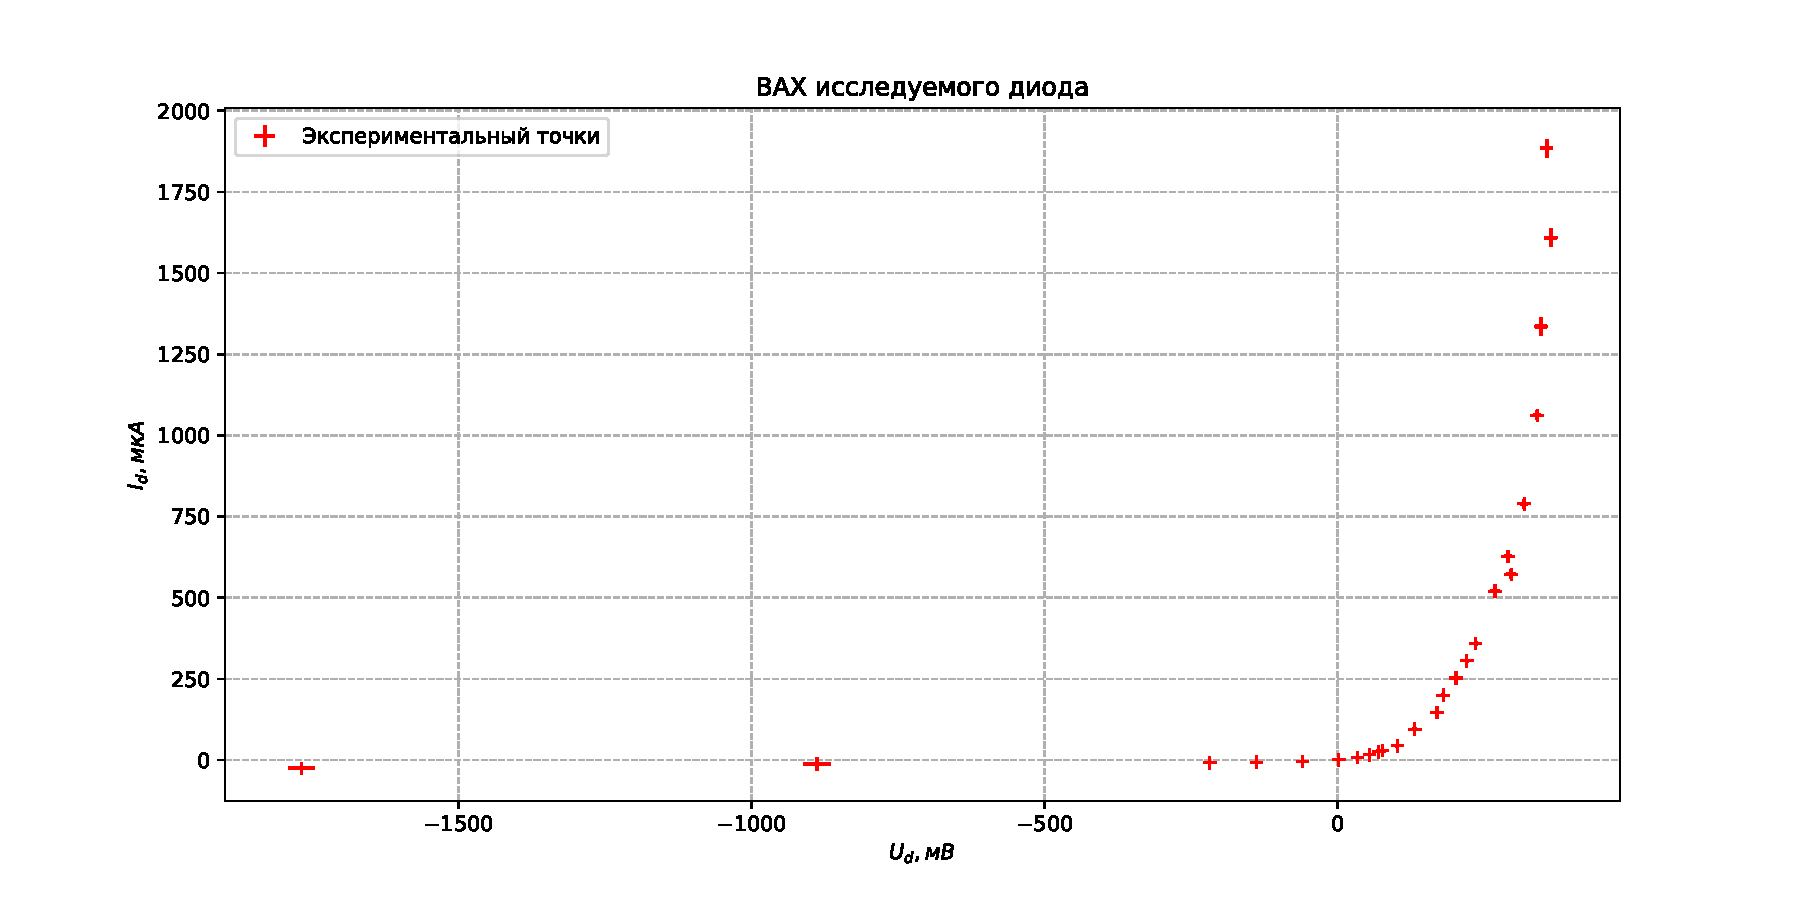
\includegraphics[width=0.78\textwidth]{pictures/VAH_diode.pdf}
    \caption{Измеренная ВАХ диода}
    \label{fig:vah}
\end{figure}

\subsection*{Измерения температурной зависимости}

Измерим зависимость сопротивления диода на линейном участке ВАХ от температуры. Все измерения при напряжении $U_0 = 25~\text{мВ}$. Результаты измерений представлены в таблице \ref{tab:main-data}. Так как нагрев непрерывный, то в процессе нагрева, но с меньшим интервалом проведем измерения по обратной части, переключаясь на $U_0 = -1 ~\text{В}$. Эти данные в таблице \ref{tab:reverse-data}.

\begin{table}[h]
    \centering
    \small
    \caption{Основные измерения при нагреве}
    \label{tab:main-data}
    \begin{tabular}{|r|r|r|r||r|r|r|r|}
        \hline
        № & $U$, мВ & $R_M$, Ом & $t$, $^\circ$C & № & $U$, мВ & $R_M$, Ом & $t$, $^\circ$C \\
        \hline
         1 & 0.03 & 620.0 & 24.29 & 14 & 1.30 & 109.0 & 54.63 \\
         2 & 0.12 & 540.0 & 26.49 & 15 & 1.39 & 100.0 & 56.71 \\
         3 & 0.20 & 470.0 & 28.44 & 16 & 1.50 &  88.0 & 59.25 \\
         4 & 0.30 & 411.0 & 30.87 & 17 & 1.60 &  77.3 & 61.55 \\
         5 & 0.40 & 358.0 & 33.29 & 18 & 1.70 &  70.0 & 63.84 \\
         6 & 0.51 & 303.0 & 35.94 & 19 & 1.80 &  62.6 & 66.12 \\
         7 & 0.60 & 264.0 & 38.11 & 20 & 1.90 &  58.1 & 68.39 \\
         8 & 0.70 & 230.0 & 40.50 & 21 & 2.02 &  52.0 & 71.10 \\
         9 & 0.81 & 196.0 & 43.11 & 22 & 2.10 &  48.0 & 72.90 \\
        10 & 0.91 & 170.0 & 45.48 & 23 & 2.20 &  45.0 & 75.13 \\
        11 & 1.00 & 154.0 & 47.61 & 24 & 2.26 &  42.0 & 76.47 \\
        12 & 1.10 & 130.0 & 49.96 & 25 & 2.30 &  41.4 & 77.36 \\
        13 & 1.20 & 120.0 & 52.30 & 26 & 2.32 &  39.0 & 77.81 \\
        \hline
    \end{tabular}
\end{table}

Из баланса моста
\begin{equation}
    R_d = 10 R_M,
\end{equation}
а погрешность сопротивления определялась как
\begin{equation}
    \sigma_{R_d} = 10 \sigma_{R_M}, \qquad \sigma_{R_M} = \SI{0.5}{\ohm}.
\end{equation}

Построим график зависимости в координатах $\ln{R_d}$ от $1 / T$. Погрешность аппроксимации определялась с помощью ODR, то есть с учётом ошибок по обеим осям. Изобразим график на рис. \ref{fig:main-fit}.

\begin{figure}[h]
    \centering
    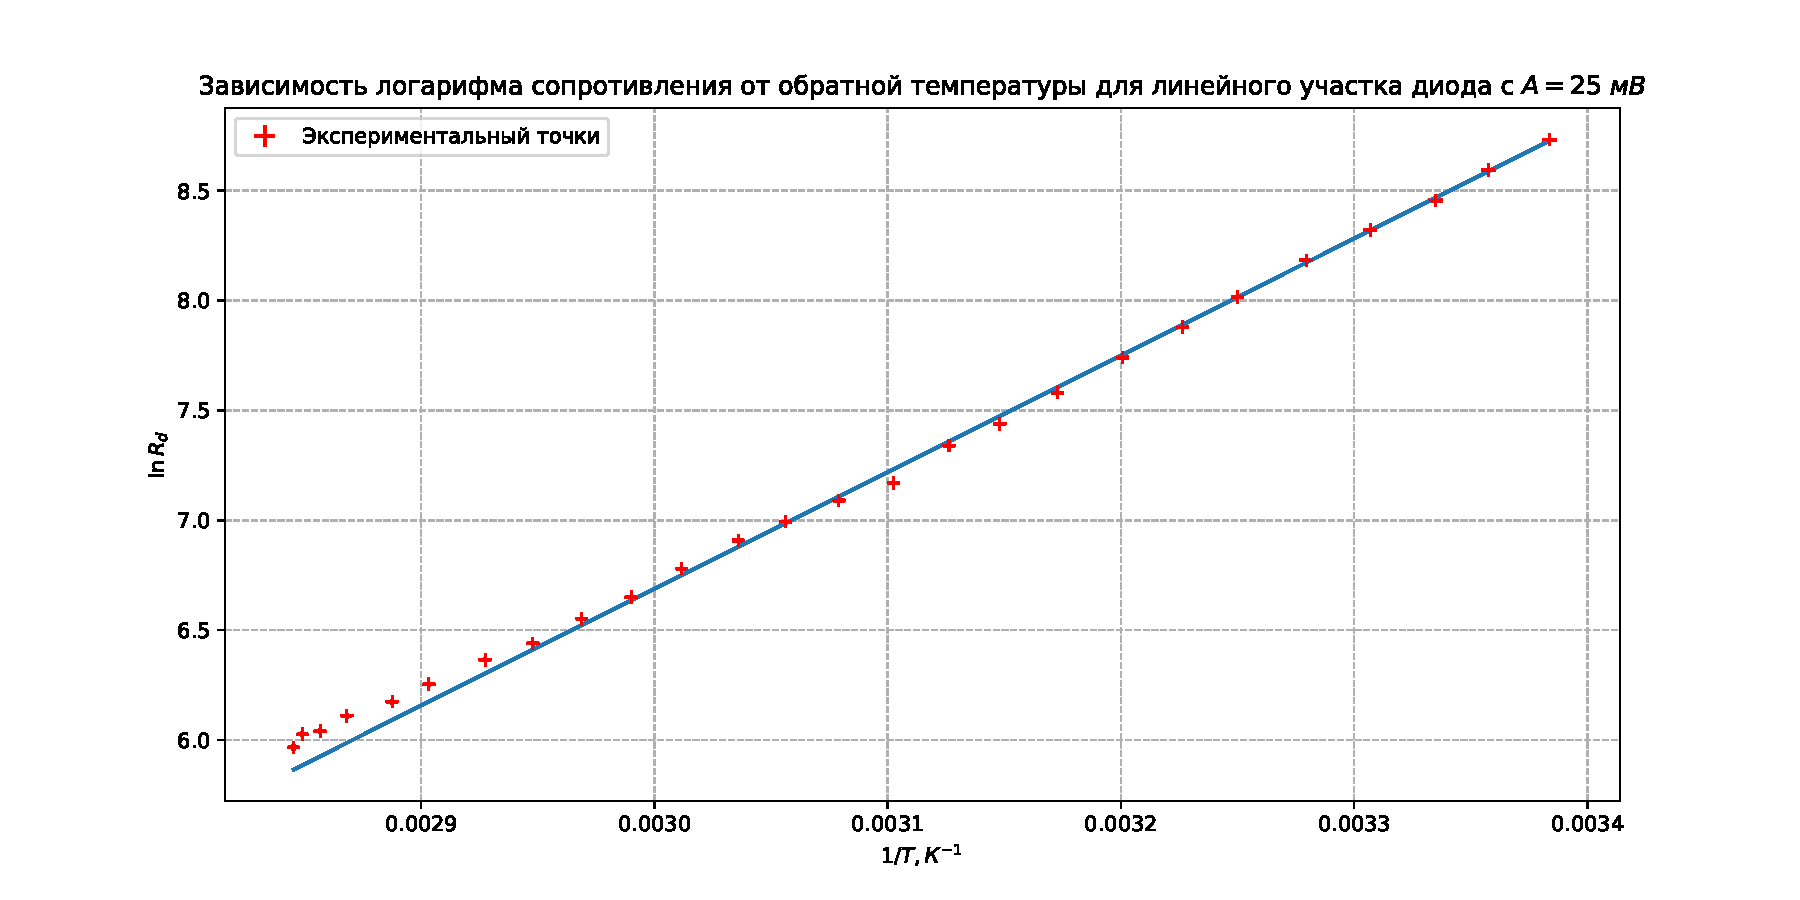
\includegraphics[width=\textwidth]{pictures/graph_straight.pdf}
    \caption{Зависимость $\ln R_d$ от $1/T$}
    \label{fig:main-fit}
\end{figure}

В результате линейной аппроксимации получено:
\begin{equation}
    \ln R_d = \frac{(537 \pm 5) \cdot 10 ~\text{К}}{T} - (9.37 \pm 0.14),
\end{equation}

Тогда из \eqref{eq:deltaV}
\begin{equation}
    \Delta V = \frac{k_{\text{Б}}}{e} k =
    (463 \pm 4)~\text{мВ}
\end{equation}


\subsection*{Оценка $\Delta V$ по обратному току}

Для семи температурных точек измерялся ток при фиксированном обратном смещении около \SI{-1}{V}. Результаты приведены в таблице \ref{tab:reverse-data}.

\begin{table}[h]
    \centering
    \small
    \caption{Измерения для обратного тока}
    \label{tab:reverse-data}
    \begin{tabular}{|r|r|r|r|r|r|}
        \hline
        № & $U$, мВ & $R_M$, Ом & $t$, $^\circ$C & $U_d$, мВ & $I_d$, мкА \\
        \hline
        1 & 0.03 & 7220.0 & 24.29 & -888.1 & -12.30 \\
        2 & 0.74 & 2570.0 & 41.45 & -738.5 & -28.74 \\
        3 & 1.04 & 1304.0 & 48.55 & -589.0 & -45.17 \\
        4 & 1.41 &  570.0 & 57.18 & -385.1 & -67.57 \\
        5 & 1.71 &  190.0 & 64.07 & -172.7 & -90.91 \\
        6 & 2.05 &   78.2 & 71.77 &  -79.1 & -101.19 \\
        7 & 2.30 &   52.0 & 77.36 &  -54.1 & -103.95 \\
        \hline
    \end{tabular}
\end{table}

По этим данным была построена зависимость $\ln |I_d|$ от $1/T$.

\begin{figure}[h]
    \centering
    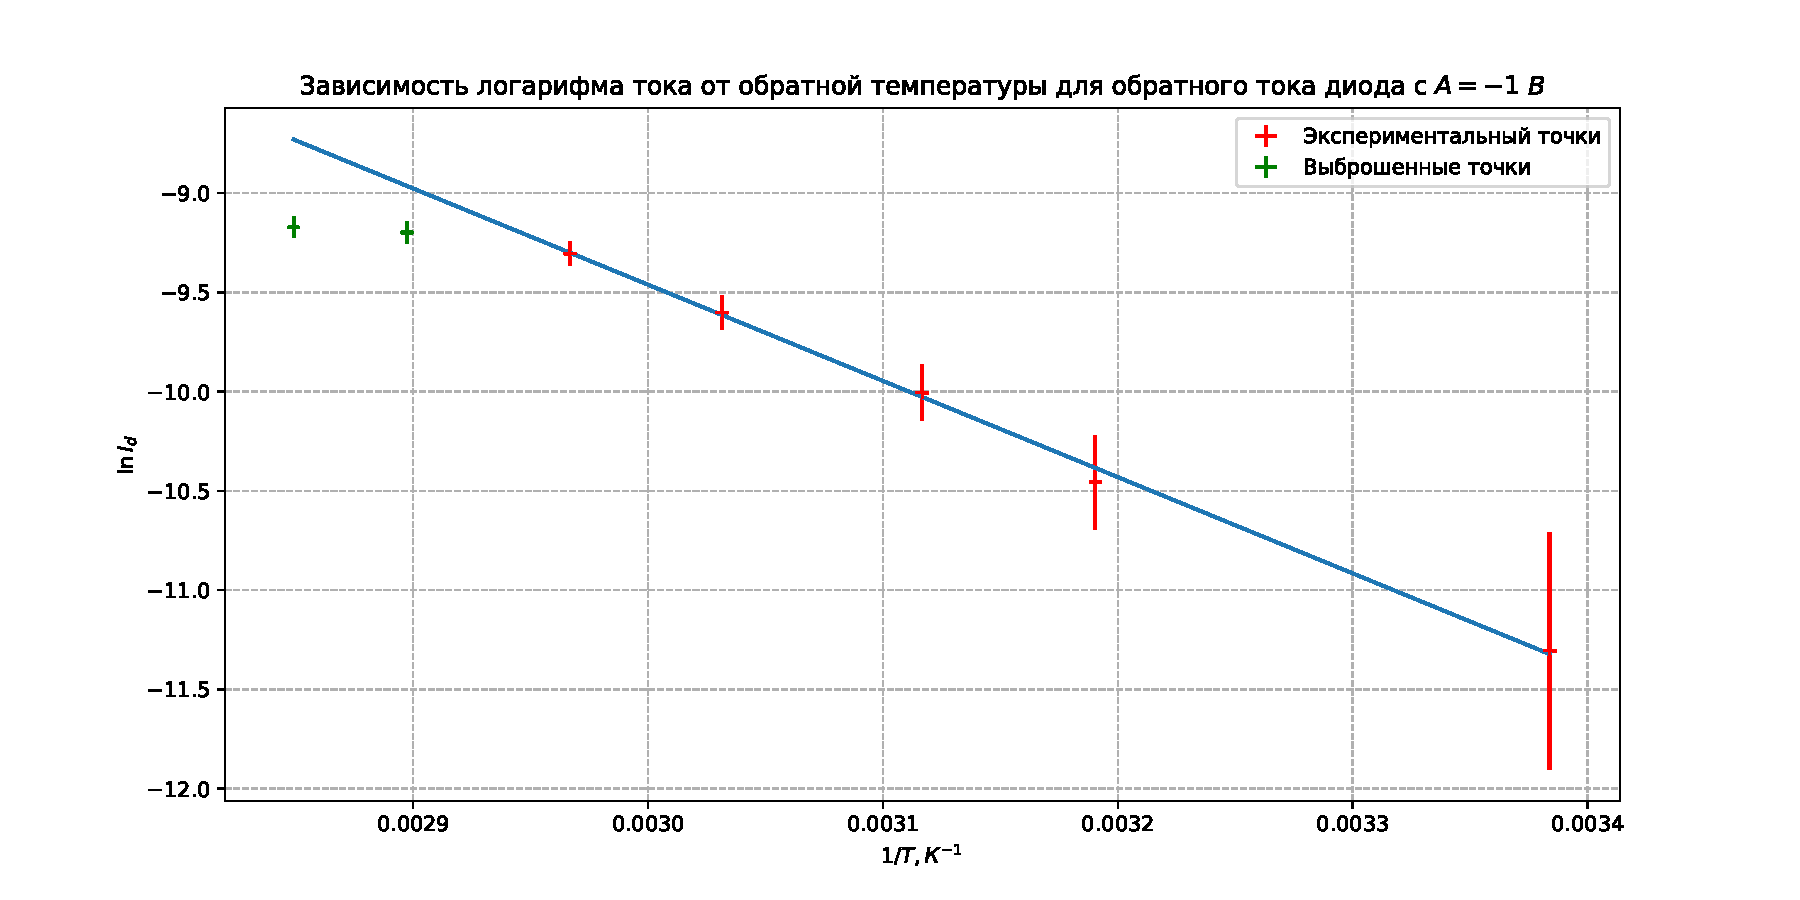
\includegraphics[width=\textwidth]{pictures/graph_reverse.pdf}
    \caption{Зависимость $\ln |I_d|$ от $1/T$ для обратного тока}
    \label{fig:reverse-fit}
\end{figure}

Взвешенная линейная аппроксимация даёт
\begin{equation}
    \ln |I_d| = -\frac{(31 \pm 4) \cdot 10^2 ~\text{К}}{T} - (0.26 \pm 1.09),
\end{equation}
откуда формально получается
\begin{equation}
    \Delta V_{\text{rev}} = (27 \pm 3) \cdot 10 ~\text{мВ}.
\end{equation}

Полученное значение отличается от значения, полученного при измерении в линейной области. 
\FloatBarrier
\section{Вывод}

\begin{itemize}
    \item Получена ВАХ исследуемого диода

    \item По температурной зависимости сопротивления $p$--$n$-перехода исследуемого диода получена контактная разность потенциалов
    \[
        \Delta V = (463 \pm 4)~\text{мВ}.
    \]

    \item Оценка по обратному току
    \[
        \Delta V_{\text{rev}} = (27 \pm 3) \cdot 10 ~\text{мВ},
    \]
\end{itemize}

Значение по обратному току может сильно отличатся из-за имеющейся большой погрешности измерений.

\end{document}
